\documentclass{beamer}
%\documentclass[handout]{beamer}


\usepackage{enumerate}
\usepackage{graphicx}
\usepackage{amsmath}
\usepackage{mathdots}
\usepackage{amsthm}
\usepackage{amssymb}
\usepackage{fancyhdr}
\usepackage{pstricks}
\usepackage{pst-node}
\pagenumbering{arabic}
\usepackage{hyperref}
\usepackage{lscape}
\usepackage{verbatim}
\usenavigationsymbolstemplate{}
\setbeamertemplate{footline}[frame number]




\title{Introduction to \LaTeX\vspace{-.5cm}}
\author{Vincent Knight\\
M1.30\\
knightva@cf.ac.uk}
\date{9/02/2012}


\begin{document}

\maketitle
\frame{\frametitle{Overview}\tableofcontents}
\section{Introduction to \LaTeX}

\frame{\frametitle{Objectives}
 Using \TeX,\;\LaTeX\; and \AmS-\LaTeX\ you will be able to
\begin{itemize}
\item Create documents containing mathematics.
\item Create presentations.
\end{itemize}\vspace{1cm}\pause


\framebox{\parbox{\textwidth}{I will not attempt to teach you everything there is to know about \LaTeX,\ (I most certainly do not know all there is to know). My goal is to teach you enough to get you started and more importantly to know where to go if you need to get further.}}
}




\frame{\frametitle{History of \LaTeX}
\parbox{\textwidth}{\emph{\textsc{``As a computer scientist, I really identify with patterns of 0's and 1's; I ought to be able to do something about this.''}}[Donald Knuth]}\vspace{1cm}

Donald Knuth was unhappy with ``state of the art'' mathematical typesetting in 1976. It took him 10 years to develop \TeX\ a document mark-up language. It is not an editor but a programming language. Since \TeX,\ various improvements have been made. Importantly each of these improvements has a different name.This means that there are no compatibility issues. \LaTeX\ is based on \TeX\ (it is a family of macros that makes using \TeX\ easier). The American Mathematical Society created a package called \AmS-\LaTeX\ that we will be using during this course.
}

\frame{\frametitle{Installing \LaTeX}
3 things are needed to be able to `\TeX' documents:
\begin{itemize}
\item A typesetting system (we will use MiKTeX)
\item A word editor (we will use TeXworks)
\item Patience
\end{itemize}
}


\frame{\frametitle{Editing Cycle}
\only<1>{\begin{center}\includegraphics[width=10cm]{Cycle}\end{center}}
\only<2>{\begin{center}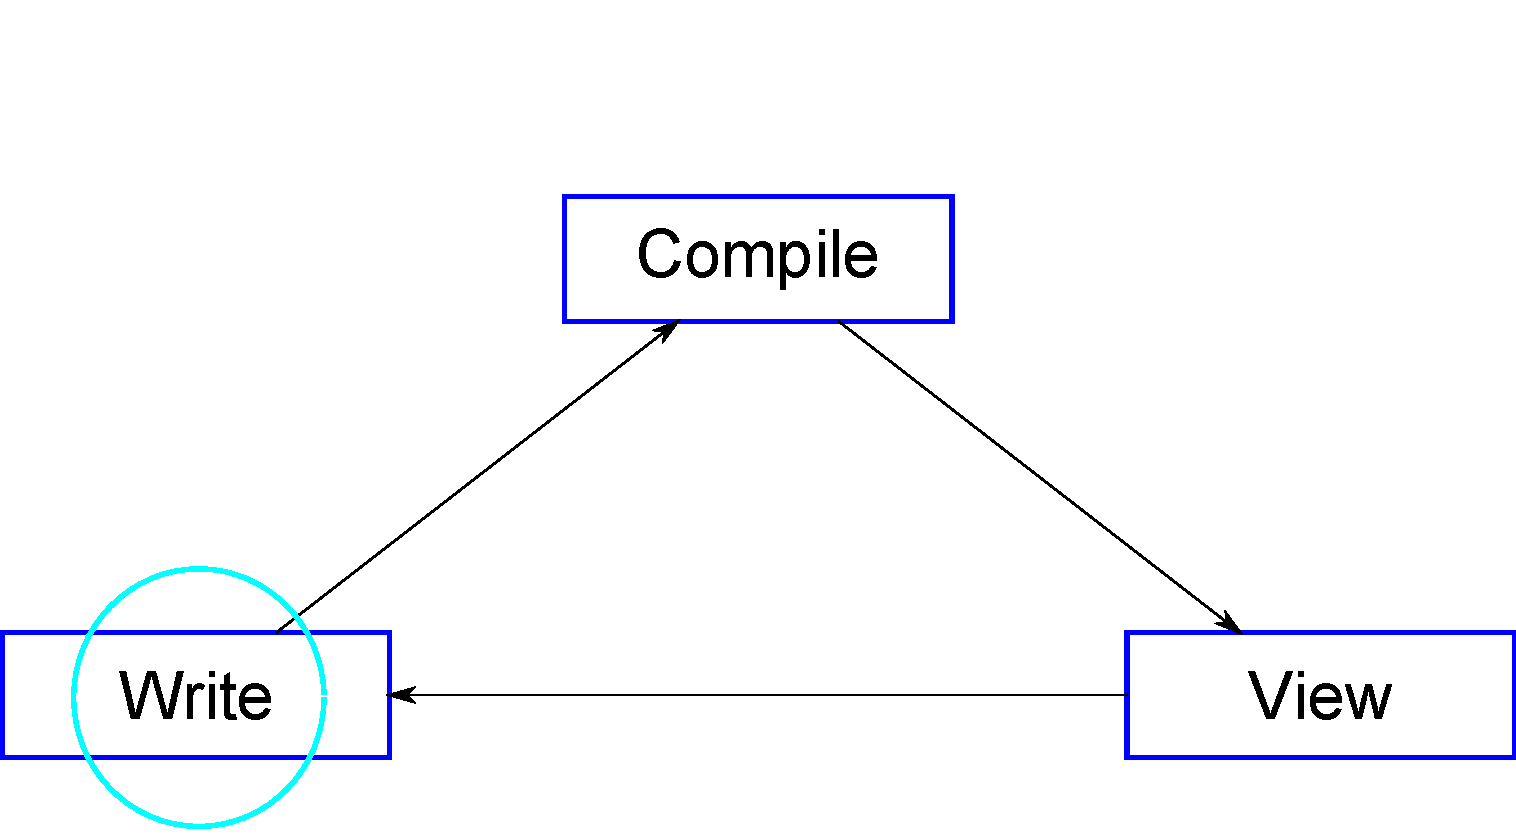
\includegraphics[width=10cm]{Write_Cycle}\end{center}}
\only<3,17>{\begin{center}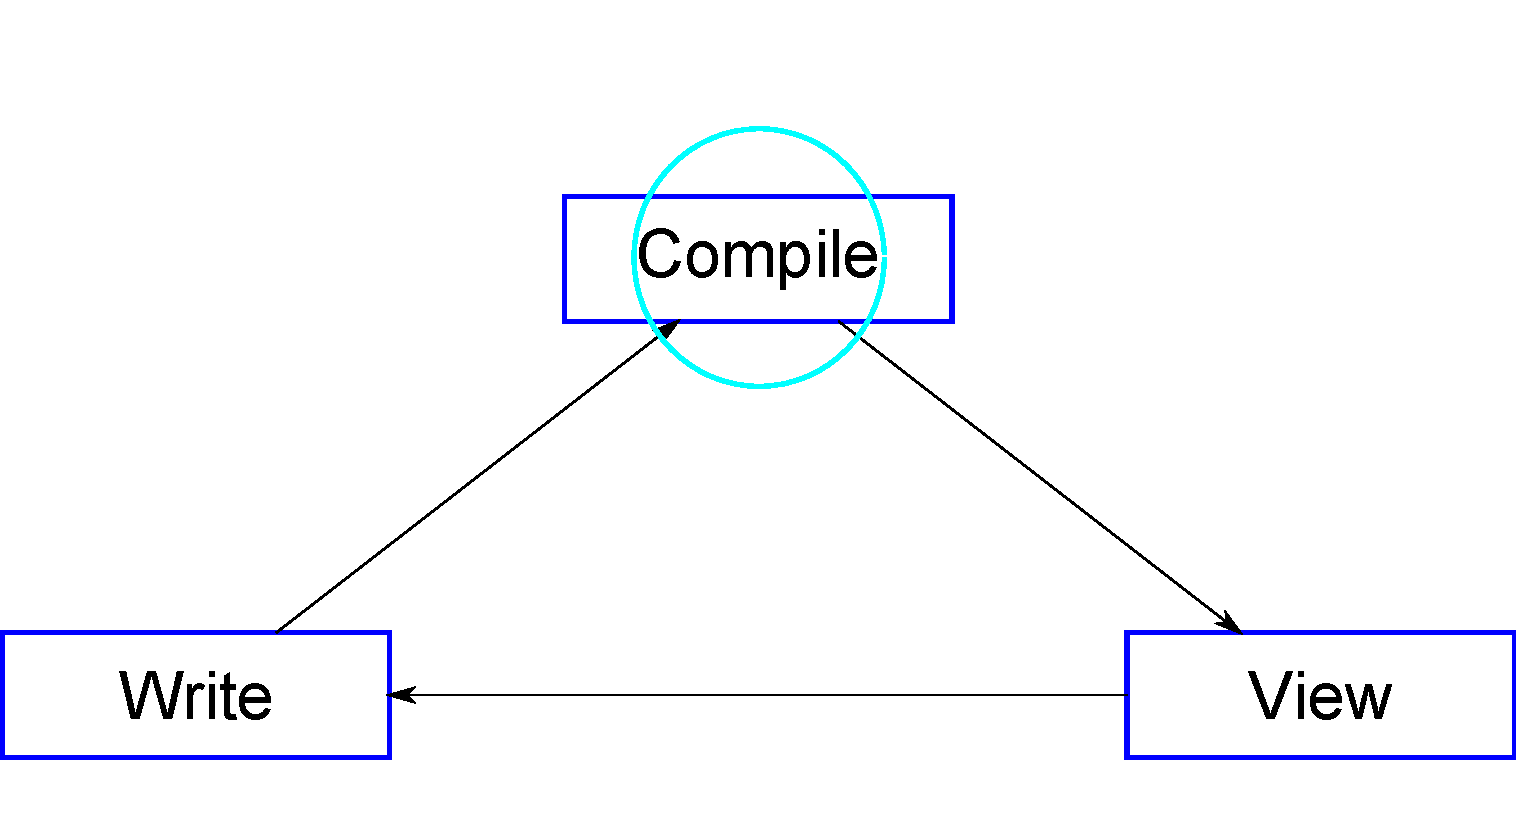
\includegraphics[width=10cm]{Compile_Cycle}\end{center}}
\only<4,18>{\begin{center}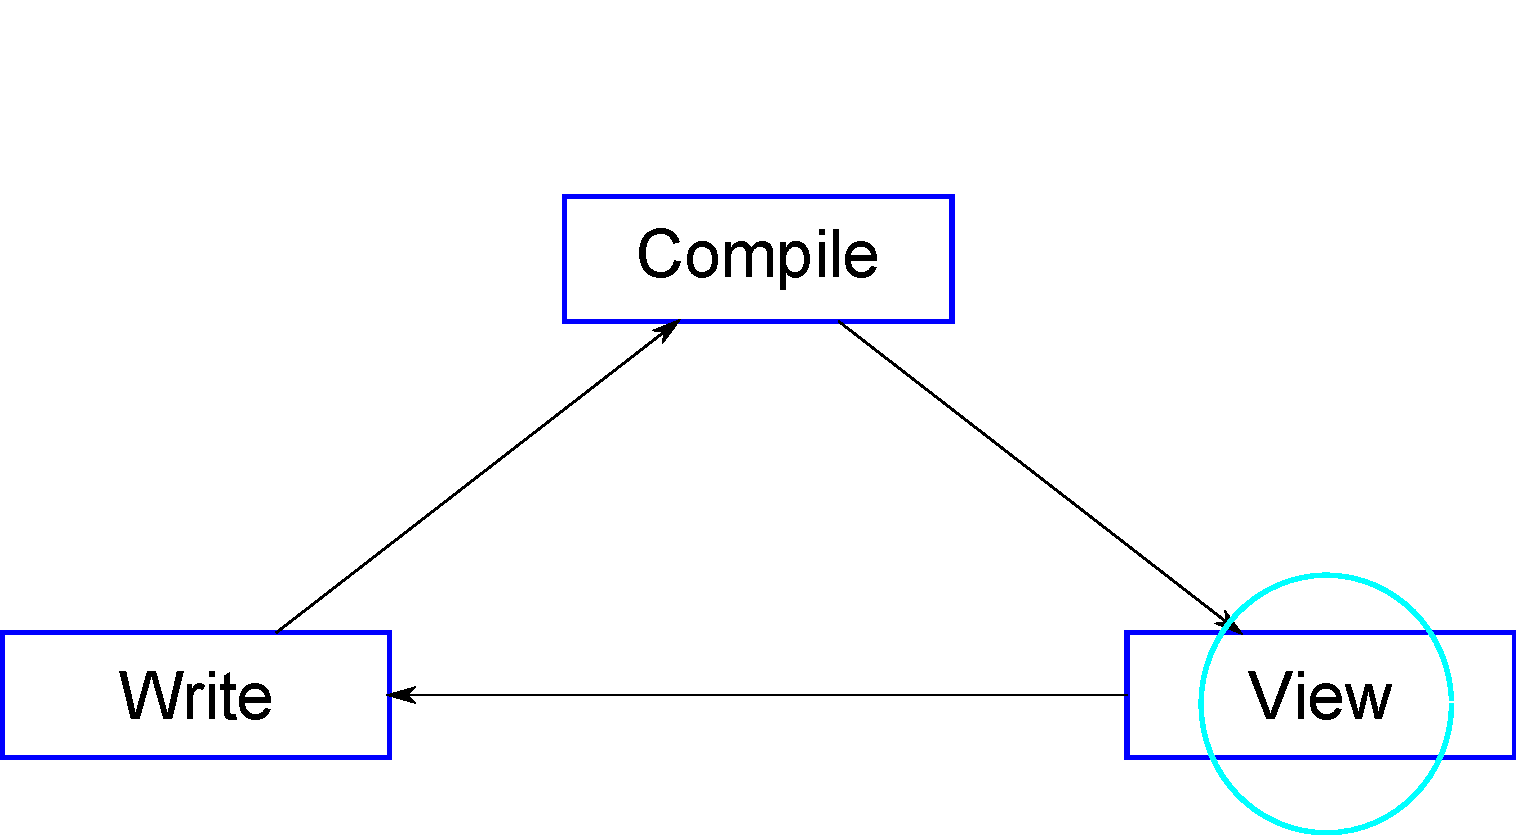
\includegraphics[width=10cm]{View_Cycle}\end{center}}
\only<5>{\begin{center}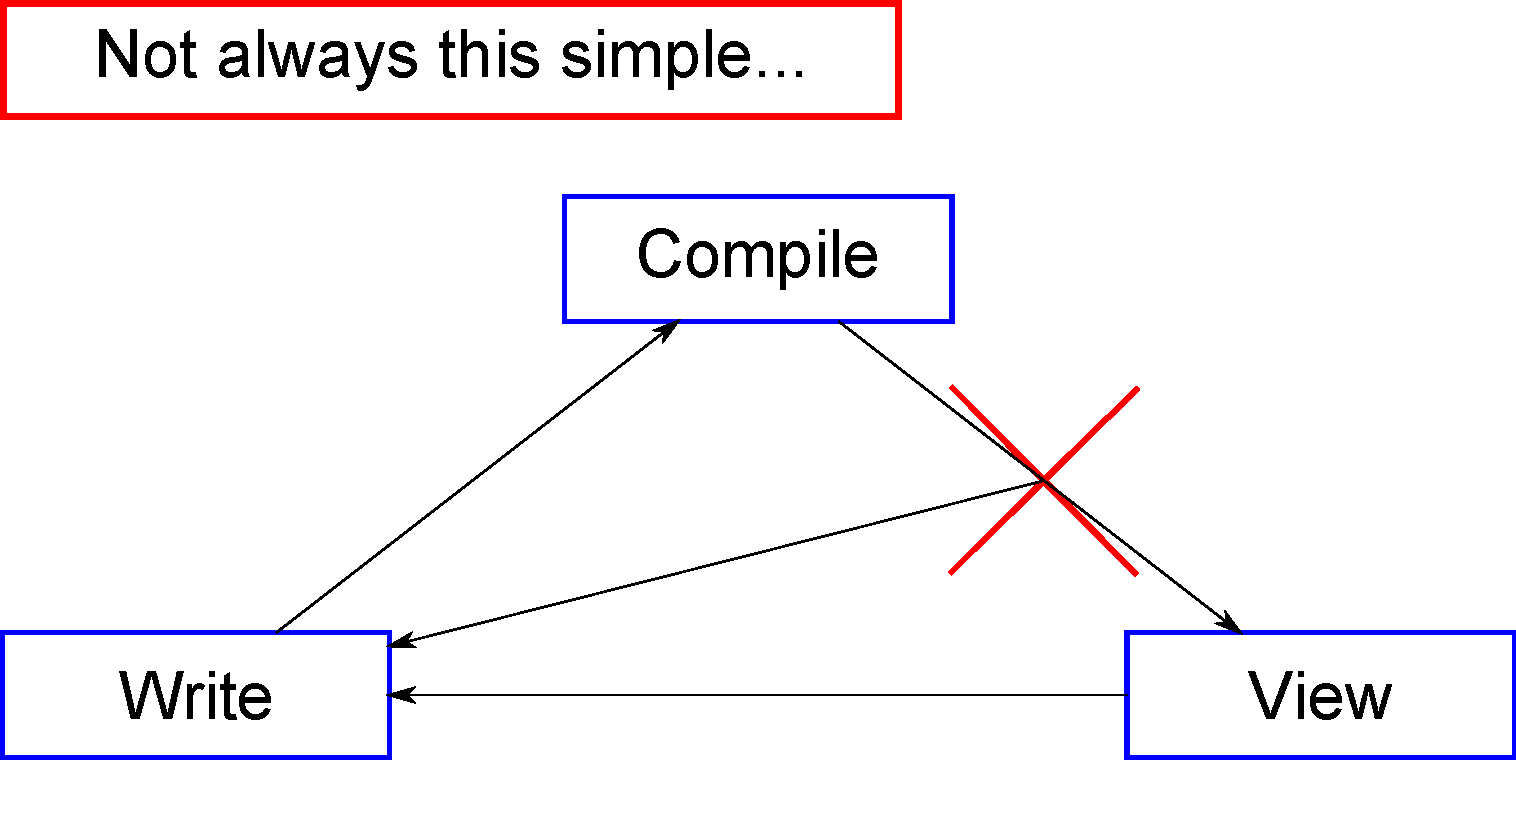
\includegraphics[width=10cm]{Broken_Cycle}\end{center}}
\only<6,9,12,15>{\begin{center}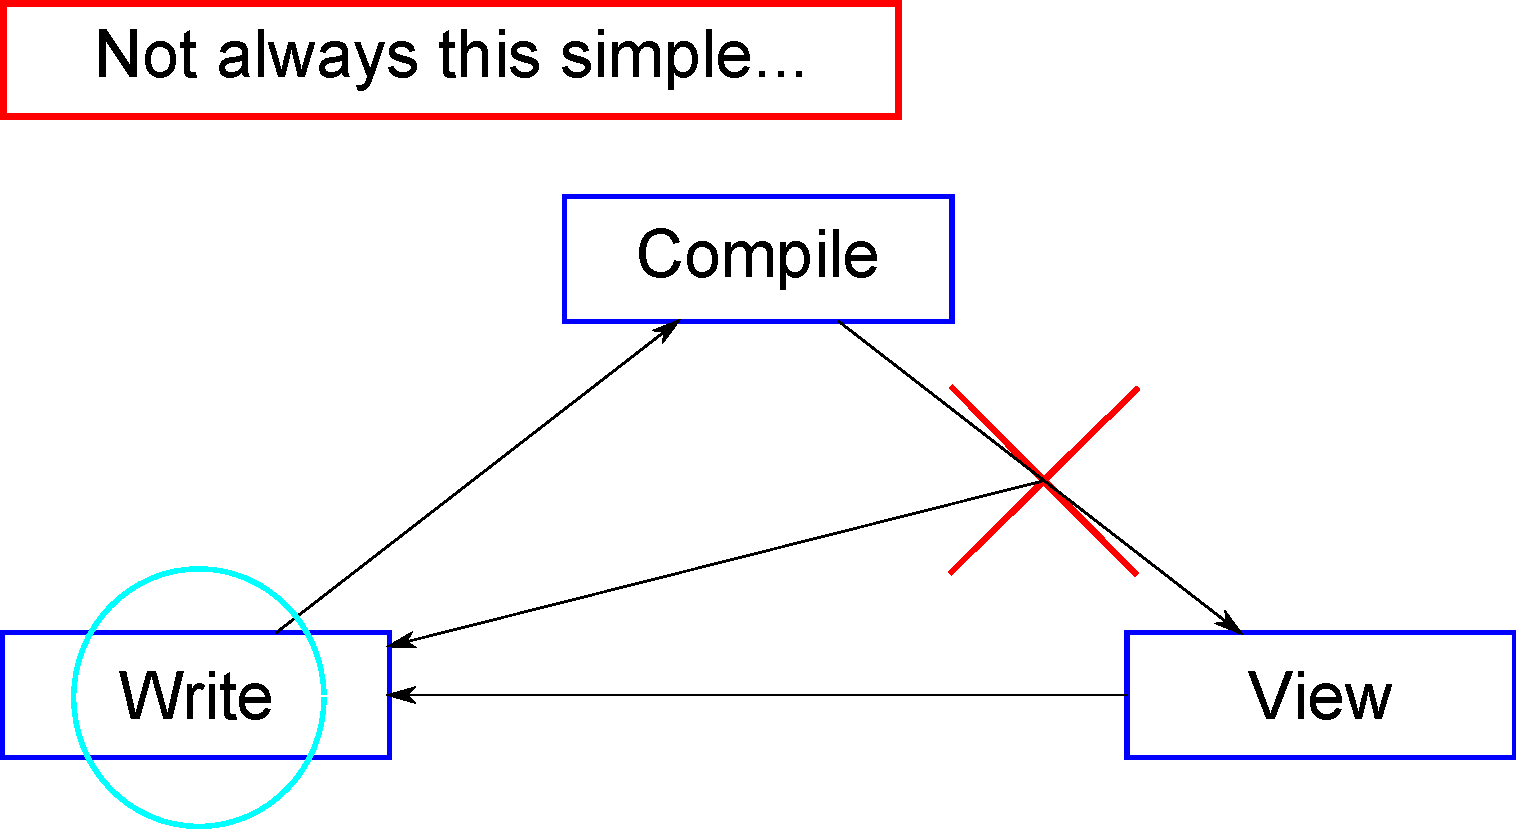
\includegraphics[width=10cm]{Write_Broken_Cycle}\end{center}}
\only<7,10,13,16>{\begin{center}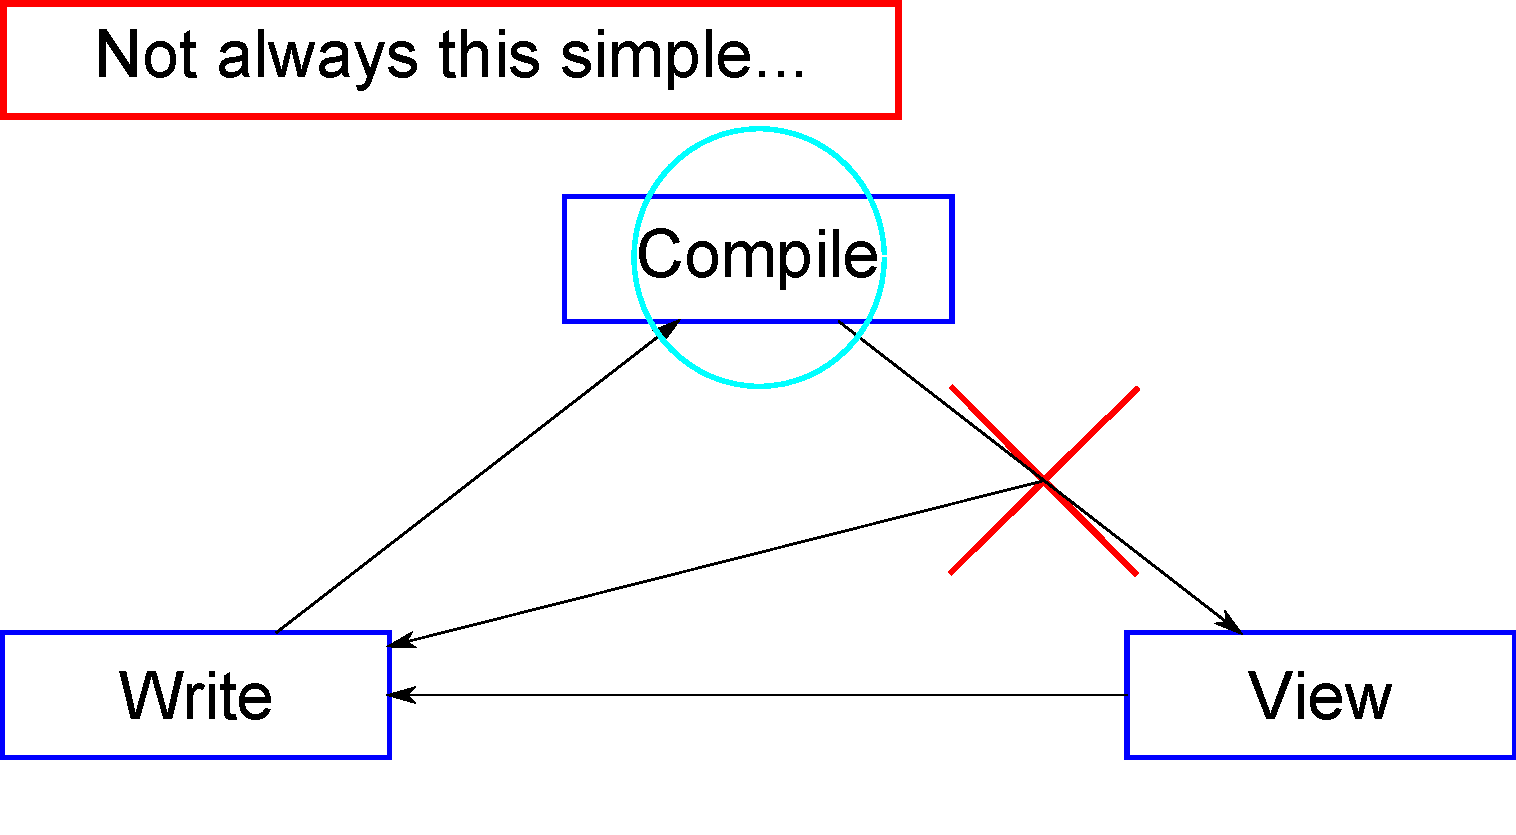
\includegraphics[width=10cm]{Compile_Broken_Cycle}\end{center}}
\only<8,11,14>{\begin{center}\includegraphics[width=10cm]{Error_Broken_Cycle}\end{center}}
%\onslide<2>{\begin{center}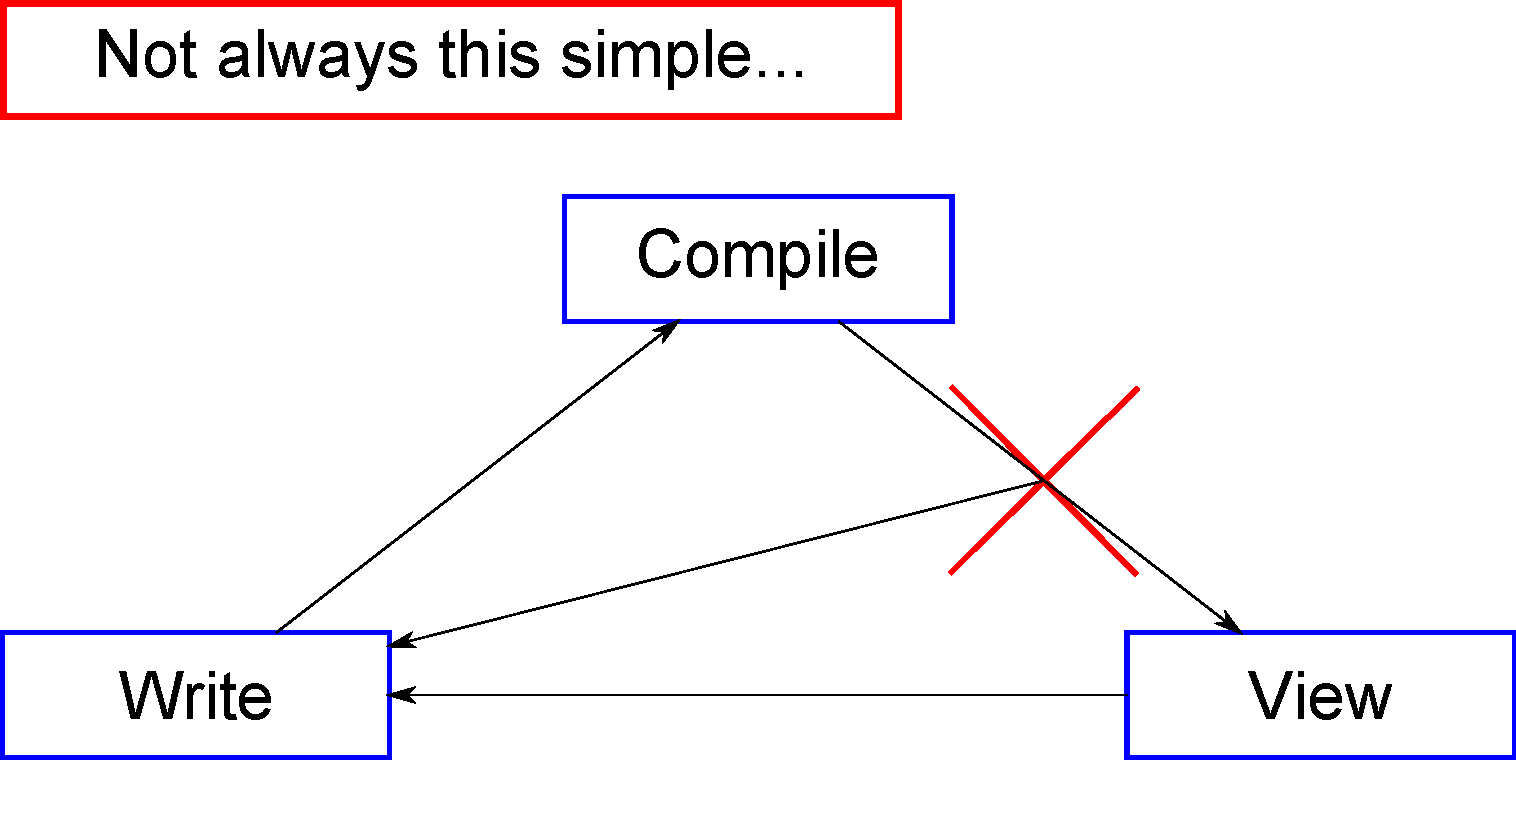
\includegraphics[width=10cm]{Broken_Cycle}\end{center}}
}

%%\frame{\frametitle{Editing Cycle}
%%
%%\begin{center}
%%\pspicture(0,0)(10,6)
%%%\psgrid(0,0)(10,6)
%%
%%\rput(2,1){\rnode{A}{\psframebox{Write}}}
%%\rput(5,5){\rnode{B}{\psframebox{Compile}}}
%%\rput(8,1){\rnode{C}{\psframebox{View}}}
%%\pnode(6.8,3){D}
%%
%%\psset{nodesep=3pt}
%%\ncarc{->}{A}{B}
%%\ncarc{->}{B}{C}
%%\ncarc{->}{C}{A}\pause
%%
%%\rput(1,5.5){\psframebox{Dislaimer: Not always easy!}}\pause
%%
%%\onslide<3>{\rput(2,1){\pscircle[linecolor=blue](0,0){1cm}}}
%%\onslide<4-5>{\rput(5,5){\pscircle[linecolor=blue](0,0){1cm}}}
%%
%%\onslide<5-15>{
%%\psline[linecolor=red](6.25,2.5)(7.25,3.5)
%%\psline[linecolor=red](6.25,3.5)(7.25,2.5)}
%%\onslide<6-7>{\rput(6.8,3){\pscircle[linecolor=blue](0,0){1cm}}}
%%\onslide<7-15>{\ncarc{->}{D}{A}}
%%\onslide<8>{\rput(2,1){\pscircle[linecolor=blue](0,0){1cm}}}
%%\onslide<9>{\rput(5,5){\pscircle[linecolor=blue](0,0){1cm}}}
%%\onslide<10>{\rput(6.8,3){\pscircle[linecolor=blue](0,0){1cm}}}
%%\onslide<11>{\rput(2,1){\pscircle[linecolor=blue](0,0){1cm}}}
%%\onslide<12>{\rput(5,5){\pscircle[linecolor=blue](0,0){1cm}}}
%%\onslide<13>{\rput(6.8,3){\pscircle[linecolor=blue](0,0){1cm}}}
%%\onslide<14>{\rput(2,1){\pscircle[linecolor=blue](0,0){1cm}}}
%%\onslide<15-16>{\rput(5,5){\pscircle[linecolor=blue](0,0){1cm}}}
%%\onslide<17>{\rput(8,1){\pscircle[linecolor=blue](0,0){1cm}}}
%%
%%\endpspicture
%%\end{center}
%%}

\frame[containsverbatim]{\frametitle{Example}
\begin{itemize}
\item Create a new document in TeXworks.
\item Save it (cheatsheet.tex).
\item Write the following code:\vspace{.5cm}

\begin{verbatim}
\documentclass{article}

\begin{document}
I can write normal text.
\end{document}
\end{verbatim}
\vspace{.5cm}
\item Ensure the dropdown window has: ``pdfLaTeX'' selected.
\item Click on the green arrow (ctrl+T).
\end{itemize}
}

\frame[containsverbatim]{\frametitle{Example}
This outputs a pdf file with the following output:
\begin{center}
\blue I can write normal text.
\end{center}
}

\frame[containsverbatim]{\frametitle{General Rules}

\begin{itemize}
\item The following keys are used to type text in a source file:
\begin{center}
a-z\;\;\;\;\;\;A-Z\;\;\;\;\;\;0-9
\end{center}
\begin{center}
+\;\;=\;\;*\;\;/\;\;(\;\;)\;\;[\;\;]
\end{center}
\item You may also use the following punctuation marks:
\begin{center}
'\;\;\;;\;\;\;.\;\;\;?\;\;\;!\;\;\;:\;\;\;`\;\;\;'\;\;\;-
\end{center}
\item Finally there are 13 special keys that are used in \LaTeX\; commands:
\begin{center}
\begin{verbatim}
             # $ % & ~ _ ^ \ { } @ " |
\end{verbatim}
\end{center}
\end{itemize}
}



\frame[containsverbatim]{\frametitle{Example}
Now attempt to add the following text:\vspace{.5cm}

\blue
I can write normal text.
\begin{center}
I can centre text.
\end{center}
\begin{flushright}
I can put text on the right.
\end{flushright}

}

\frame[containsverbatim]{\frametitle{Example}

\begin{verbatim}
\documentclass{article}

\begin{document}
I can write normal text.

\begin{center}
I can centre text.
\end{center}

\begin{flushright}
I can put text on the right.
\end{flushright}

\end{document}
\end{verbatim}
}

\frame[containsverbatim]{\frametitle{\LaTeX\ Structure}

\red\scriptsize\begin{verbatim}

\documentclass{...}
\usepackage{...}
...

\begin{document}

\title{...}
\author{...}
\date{...}


\maketitle

\begin{abstract}
...
\end{abstract}

\section{...}
\section{...}

\newpage
\pagestyle{...}
\bibliographystyle{...}
\bibliography{...}
\end{document}

\end{verbatim}

%\normalsize\black
%\rput(8.9,9){$\left.\pspicture(0,0)(0,.5)\endpspicture\right\}$Preamble}
%\rput(8.6,4.4){$\left.\pspicture(0,0)(0,3.1)\endpspicture\right\}$Body}
%\rput(6.5,5.7){$\left.\pspicture(0,0)(0,1.8)\endpspicture\right\}$Top Matter}
%\rput(6.6,3.4){$\left.\pspicture(0,0)(0,.4)\endpspicture\right\}$Main Matter}
%\rput(6.6,1.8){$\left.\pspicture(0,0)(0,.6)\endpspicture\right\}$Back Matter}
%\rput(4,4.4){$\left.\pspicture(0,0)(0,.5)\endpspicture\right\}$Abstract}
}

\frame[containsverbatim]{\frametitle{\LaTeX\ Structure}
\blue\begin{verbatim}
\documentclass{...}
\end{verbatim}
\black This command takes an argument that defines the type of document we want to produce. Some of the most common are listed below:
\begin{itemize}
\item article (very common)
\item report
\item letter
\item book
\item beamer (this is what was used to make these slides)
\end{itemize}
It is also possible to create your own. This is often done by publishers who simply provide you with their own class file.
}

\frame[containsverbatim]{\frametitle{\LaTeX\ Structure}
\begin{verbatim}
\usepackage{...}
\end{verbatim}
\black The is a very important command that calls external macros. Common packages are listed below:
\begin{itemize}
\item amsmath (very useful)
\item hyperref
\item mathdots
\item enumerate
\end{itemize}
Once again it is possible to create your own.
}


\frame[containsverbatim]{\frametitle{Structure}
Create the following title for your cheatsheet:\\

\begin{verbatim}
\title{ \LaTeX\ cheatsheet}
\author{Your Name}
\date{\today}
\end{verbatim}

Importantly include the following code to actually include the title:
\begin{verbatim}
\maketitle
\end{verbatim}
}

\frame[containsverbatim]{\frametitle{\LaTeX\ Structure}
Add the following abstract to your cheatsheet:\\

\begin{verbatim}
\begin{abstract}

This document will be useful to me as a
\textbf{reference} document from which
I can start all my future \LaTeX\ files.

\end{abstract}
\end{verbatim}
}


\frame[containsverbatim]{\frametitle{Text Sizes}
\begin{columns}
\column{.5\textwidth}
\begin{center}
\begin{verbatim}
\tiny
\scriptsize
\small
\normalsize
\large
\Large
\huge
\Huge
\end{verbatim}
\end{center}
\column{.5\textwidth}
\begin{center}
\tiny Text\\
\scriptsize Text\\
\small Text\\
\normalsize Text\\
\large Text\\
\Large Text\\
\huge Text\\
\Huge Text
\end{center}
\end{columns}
}

\frame[containsverbatim]{\frametitle{\LaTeX\ Structure}
Add the following line of code to your cheetsheet:\\

\begin{verbatim}


\begin{center}
\tiny Text\\
\scriptsize Text\\
\small Text\\
\normalsize Text\\
\large Text\\
\Large Text\\
\huge Text\\
\Huge Text
\end{center}


\end{verbatim}
}

\frame[containsverbatim]{\frametitle{Spacing}
There are various ways of of handling spacing in \LaTeX.
\begin{itemize}
\item The \verb'\\' command ends a line.
\item Horizontal spaces can be added using \verb \  ,\verb \: ,  \verb \; or \verb'\hspace{length}'.
\item Vertical spaces can be added using \verb'\vspace{length}'.
\end{itemize}
where \verb'length' is a multiple of one of the following units:
\begin{center}

\begin{tabular}{|c|c|}
\hline
\verb'pt'&a point is about 0.3515mm\\\hline
\verb'bp'&a big point is about 0.3527mm\\\hline
\verb'mm'&a millimeter\\\hline
\verb'cm'&a centimeter\\\hline
\verb'in'&an inch\\\hline
\verb'ex'&roughly the height of an 'x' in the current font\\\hline
\verb'em'&roughly the height of an 'M' in the current font\\\hline
\end{tabular}
\end{center}
}

\frame[containsverbatim]{\frametitle{Page Formatting}
It is very simple in \LaTeX\ to control your page formatting. Experiment with the following code in your preamble.

\begin{verbatim}

\setlength{\textheight}{240mm}
\setlength{\textwidth}{166mm}
\setlength{\topmargin}{0mm}
\setlength{\oddsidemargin}{0mm}

\end{verbatim}
}

\frame[containsverbatim]{\frametitle{Line Spacing}
To deal with line spacing, include the ``setspace'' package to your preamble (\verb'\usepackage{setspace}'). Then experiment with the following commands.

\begin{verbatim}

\singlespacing
\doublespacing
\onehalfspacing

\end{verbatim}
}


\frame[containsverbatim]{\frametitle{Paragraph Formatting}
We can format the indentation and spacing of paragraphs using the following commands:
\begin{verbatim}

\setlength{\parindent}{0mm}
\setlength{\parskip}{0mm}

\end{verbatim}
}

\frame[containsverbatim]{\frametitle{Lists}
There are various ways to list elements in \LaTeX. Experiment with the following code in your cheatsheet:
\begin{verbatim}
There are various ways to have lists in \Latex\:

\begin{itemize}
\item Like
\item This
\end{itemize}

or

\begin{enumerate}
\item Like
\item This
\end{enumerate}
\end{verbatim}
}

\frame[containsverbatim]{\frametitle{Bibliographies, Sections and Figures}
We will now see how to include and refer to:
\begin{itemize}
\item Tables
\item Bibliographies
\item Sections
\item Figures
\end{itemize}
Importantly these can all be referenced very easily using the \verb'\label{...}' and \verb'\ref{...}' commands.
}

\frame[containsverbatim]{\frametitle{pdfLaTex+MakeIndex+BibTeX}
\begin{center}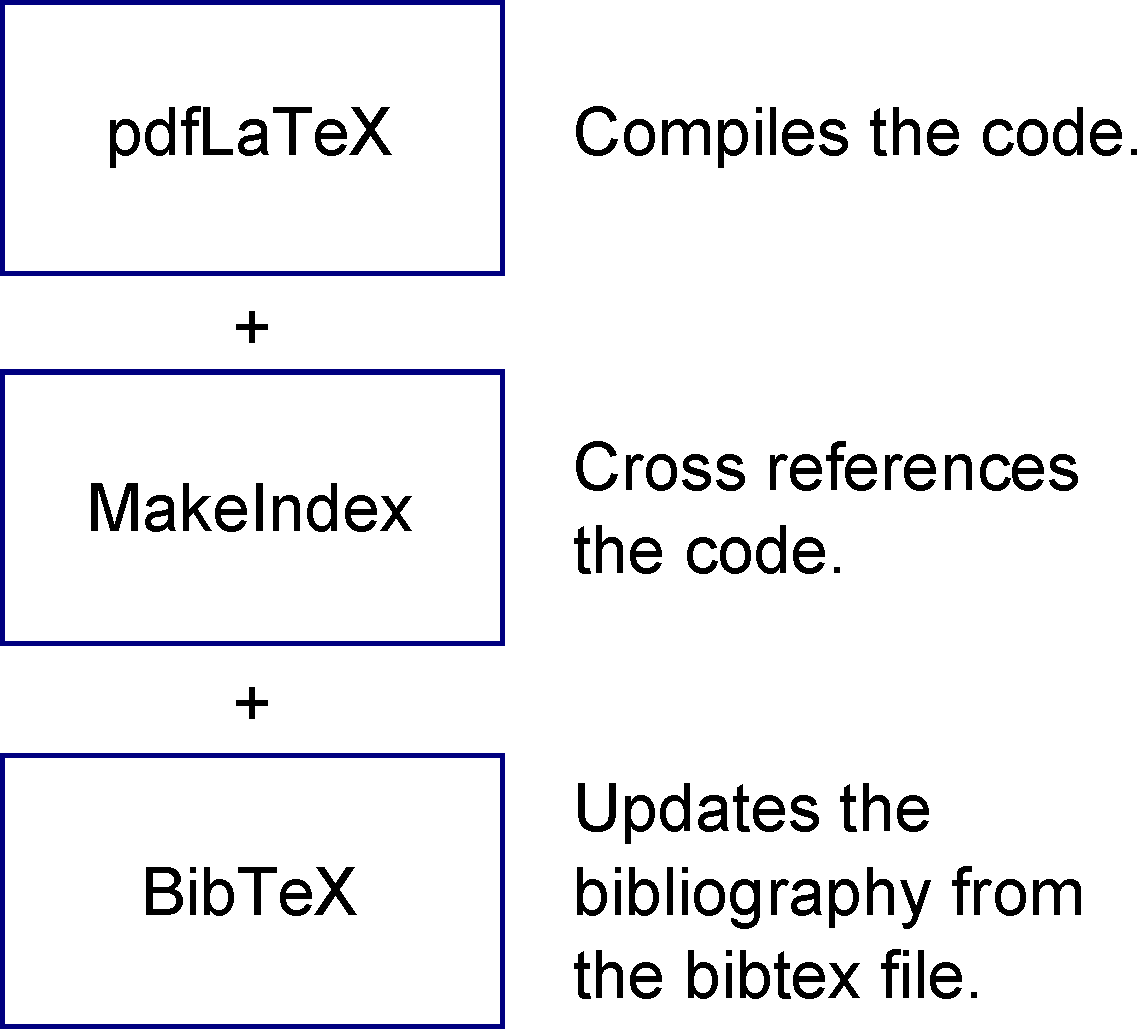
\includegraphics[width=6cm]{pdfLaTex+MakeIndex+BibTeX}\end{center}
}


\frame[containsverbatim]{\frametitle{Tables}
Tables are created using the tabular and table environment.
\begin{verbatim}
\begin{table}
\begin{tabular}{|c|c|c|}
\hline
Names&Gender&Start Time\\
\hline
Angelico&Male&1100\\
\hline
Leanne&Female&0830\\
\hline
Lisa&Female&0730\\
\hline
Paul&Male&0730\\
\hline
\end{tabular}
\caption{My Table}\label{My_Table}
\end{table}
\end{verbatim}
}

\frame[containsverbatim]{\frametitle{Tables}
\begin{center}
\blue
\begin{table}
\begin{tabular}{|c|c|c|}
\hline
Names&Gender&Start Time\\
\hline
Angelico&Male&1100\\
\hline
Leanne&Female&0830\\
\hline
Lisa&Female&0730\\
\hline
Paul&Male&0730\\
\hline
\end{tabular}
\caption{My Table}\label{My_Table}
\end{table}
\end{center}
}


\frame[containsverbatim]{\frametitle{Bibliographies}
\LaTeX\ handles bibliographies using 2 tools:
\begin{itemize}
\item A \emph{bibtex} file that stores all your references.
\item The \verb'\cite{...}' command.
\end{itemize}
Create a new file in texworks and write the following code:
\begin{verbatim}
@book{Gratzer2007,
author = {Gr\"{a}tzer, George},
publisher = {Springer},
title = {{More Math Into LaTeX: A Guide for
	          Documentation and Presentation}},
year = {2007}
}
\end{verbatim}
Save this file as a bibtex file (Myfirstbibfile.bib).
}

\frame[containsverbatim]{\frametitle{Bibliographies}
To reference a document simply call it in by using its `citation key' and the command \verb'\cite{...}'. Add the following code to your cheat sheet:
\begin{verbatim}
A very helpful reference for
\LaTeX\ is \cite{Gratzer2007}.
\end{verbatim}
Finally point your cheat sheet in the direction of your bibtex file by using the following code:
\begin{verbatim}
\newpage
\bibliographystyle{plain}
\bibliography{Myfirstbibfile}
\end{verbatim}
To compile your bibliography you must ensure that you use bibtex as well as pdflatex.
}




\frame[containsverbatim]{\frametitle{Sections}
Documents can be further fragmented using the sections command:
\begin{verbatim}
\section{...}
\subsection{...}
\subsubsection{...}
\end{verbatim}
}

\frame[containsverbatim]{\frametitle{Sections}
Include a label to your first section (\verb'\label{General_Typesetting}') and add the following code to your cheat sheet:
\begin{verbatim}
\section{Typesetting Mathematics}
In Section \ref{General_Typesetting} we saw how to type
general text. We will now type mathematics.
\end{verbatim}
Finally include a table of contents by using:
 \verb'\tableofcontents'
}


\frame[containsverbatim]{\frametitle{Inserting Figures}
Inserting figures in to a \LaTeX\ document is also very simple (using pdf-\LaTeX) using the `graphicx' package. Simply ensure that your figure (for the purpose of this exercise go find a jpg of your choice from the internet) is located in the same folder as your \LaTeX document and use the following code (as well as including \verb'\usepackage{graphicx}' in your preamble):

\begin{verbatim}

\begin{figure}[h]
\begin{center}

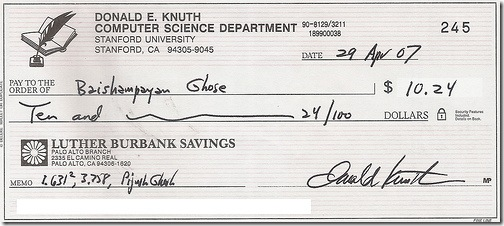
\includegraphics[width=10cm]{picture}

\caption{My first picture in \LaTeX.}\label{pic_fig}
\end{center}
\end{figure}

It is good to see that we can reference
figures like this: Figure \ref{pic_fig}.
\end{verbatim}
}

\frame[containsverbatim]{\frametitle{Inserting Figures}
Note that the compilation engine you use has an effect on what format of picture you may use:

\begin{center}
\begin{tabular}{c|c}
Compiler& Compatible Image Files\\
\hline
pdf\LaTeX&JPG, PNG, PDF\\
\LaTeX&Encapsulated PostScript (EPS)\\
Xe\LaTeX&(All?)
\end{tabular}
\end{center}
}

\frame[containsverbatim]{\frametitle{Vector Graphics}
There are two types of ``pictures":
\begin{itemize}
\item Bitmaps (JPG, PNG,etc...)
\item Vector graphics (EPS,PDF,SVG,...)
\end{itemize}
The latter allows for a better scaling of images:
\begin{center}
\begin{tabular}{|l|c|c|}
\hline
&Bitmap&Vector Graphics\\\hline
Original&
\includegraphics{dotpngpic}&
\includegraphics{dotpdfpic}\\
\hline
Scaled&
\includegraphics[width=3cm]{dotpngpic}&
\includegraphics[width=3cm]{dotpdfpic}\\
\hline
\end{tabular}
\end{center}
}



\section{Mathematics in \LaTeX}
\frame{\frametitle{Typesetting mathematics}
\parbox{\textwidth}{\emph{\textsc{``The hardest thing is to go to sleep at night, when there are so many urgent things needing to be done. A huge gap exists between what we know is possible with today's machines and what we have so far been able to finish.''}}[Donald Knuth]}\vspace{1cm}
Typesetting mathematics is \LaTeX's strength. We will concentrate on the building blocks. These allow us to build very complicated formulae. Concentrate selectively on the ones you need.
}

\frame[containsverbatim]{\frametitle{Math in text}
Math in text (\emph{inline}) is enclosed by \verb'$' symbols (or by \verb'\(' and \verb'\)'). Add the following code to your cheatsheet:
\begin{verbatim}
Mathematics can be typed in to \LaTeX\ as $x^2$
and/or \((a+b)^2=a^2+2ab+b^2\).
\end{verbatim}

}

\frame[containsverbatim]{\frametitle{Math in text}
\blue Mathematics can be typed in to \LaTeX\ as $x^2$
and/or \((a+b)^2=a^2+2ab+b^2\).

}

\frame[containsverbatim]{\frametitle{Displayed Mathematics}
Math in display mode is enclosed by \verb'$$' symbols (or by \verb'\[' and \verb'])'). Add the following code to your cheatsheet:
\begin{verbatim}
It is sometimes nicer to display more
complex formula like this:
$$\sum_{i=1}^ni={n(n+1)\over 2}$$
and
\[\int_{0}^nxdx={n^2\over2}\]
\end{verbatim}
}

\frame[containsverbatim]{\frametitle{Displayed Mathematics}
It is sometimes nicer to display more
complex formula like this:
$$\sum_{i=1}^ni={n(n+1)\over 2}$$
and
\[\int_{0}^nxdx={n^2\over2}\]
}


\frame[containsverbatim]{\frametitle{Displayed Mathematics}
It is also possible to display mathematics as equations that can be referred to later.
\begin{verbatim}
\begin{equation}\label{my_first_equation}
e=mc^2
\end{equation}


In equation (\ref{my_first_equation}) we
have a very well known relationship!
\end{verbatim}
}

\frame[containsverbatim]{\frametitle{Text in Maths}
Sometimes you might want to include texts in math statements. This can be done easily thanks to the  \AmS-\LaTeX\ package and the \verb'\text' command. Attempt the following code:
\begin{verbatim}
\[x^2=1\text{ implies }x=\pm1\]
\end{verbatim}
Try the same code without the \verb'text' function.\\
(Another option is \verb'\mbox')
}


\frame[containsverbatim]{\frametitle{Arithmetic}
Arithmetic operations are quite simple in \LaTeX. Try the following code.
\begin{verbatim}
\subsection{Arithmetic}

\begin{itemize}
\item $a+b$
\item $a-b$
\item $-a$
\item $ab$
\item $a\cdot b$
\item $a\times b$
\item $a/b$
\item ${a\over b}$
\item $\frac{a}{b}$
\end{itemize}
\end{verbatim}
}

\frame[containsverbatim]{\frametitle{Arithmetic}
Subscripts and superscripts are obtained with the following code:
\begin{verbatim}
Some examples of subscripts and superscripts:
\begin{itemize}
\item $a_{k}$
\item $b^{2}$
\item $a_{b^{2}}$
\item $a^{b^{c}}$
\end{itemize}
\end{verbatim}
}

\frame[containsverbatim]{\frametitle{Integrals}
Experiment with the following code
\begin{verbatim}
\subsection{Integrals}

$$\int_{0}^{\pi}x^2\,dx$$

\end{verbatim}
}



\frame[containsverbatim]{\frametitle{Binomial Coefficients}
Binomial coefficients (such as ${n\choose 2}$ are obtained with the following code:
\begin{verbatim}
\subsection{Binomial Coefficients}

\begin{itemize}
\item ${n\choose 2}$
\item $\binom{r^2}{a}$
\end{itemize}
\end{verbatim}
}

\frame[containsverbatim]{\frametitle{Congruences}
Congruence equations such as:
$$7\equiv 3\pmod 4$$
or
$$2001\equiv 0\pod 3$$

 are obtained with the following code:
\begin{verbatim}

\subsection{Congruences}

\begin{itemize}
\item $7\equiv 3\pmod 4$
\item $2001\equiv 0\pod 3$
\end{itemize}
\end{verbatim}
}

\frame[containsverbatim]{\frametitle{Delimeters}
Parentheses and square brackets are very easy to obtain in \LaTeX. Experiment with the following code:

\begin{verbatim}
\subsection{Delimiters}

 $$(\int_{0}^y{1+x\over 2+y}\,dy)$$
 $$\left(\int_{0}^y{1+x\over 2+y}\,dy\right)$$
 $$\left[\int_{0}^y{1+x\over 2+y}\,dy\right]$$
 $$\left|\int_{0}^y{1+x\over 2+y}\,dy\right|$$
 $$\left\|\int_{0}^y{1+x\over 2+y}\, dy\right\|$$
\end{verbatim}
}

\frame[containsverbatim]{\frametitle{Ellipsis}
The \emph{ellipsis} (...) in text is provided by the \verb'\dots' command.

\begin{verbatim}
\subsection{Ellipsis}

 $$A\dots Z$$
 $$F(x_1,\dots,x_n)$$
 $$x_1+\dots+x_n$$
\end{verbatim}
}

\frame[containsverbatim]{\frametitle{Ellipsis}

\blue
 $$A\dots Z$$
 $$F(x_1,\dots,x_n)$$
 $$x_1+\dots+x_n$$
}

\frame[containsverbatim]{\frametitle{Math Accents}
Experiment with the following code
\begin{verbatim}
\subsection{Math Accents}

\begin{enumerate}
\item $\bar{a}$
\item $\hat{a}$
\item $\tilde{a}$
\item $\vec{a}$
\end{enumerate}


\end{verbatim}
}


\frame[containsverbatim]{\frametitle{Matrices}
The matrix:
$$\begin{matrix}
a+b+c&uv&x-y\\
a+b&u+v&z\\
\end{matrix}$$
is typed with the following code:
\begin{verbatim}
\subsection{Matrices}

$$\begin{matrix}
a+b+c&uv&x-y\\
a+b&u+v&z\\
\end{matrix}$$
\end{verbatim}
}

\frame[containsverbatim]{\frametitle{Matrices}
The matrix:
$$\begin{pmatrix}
a&b\\
c&d\\
e&f\\
\end{pmatrix}$$
is typed with the following code:
\begin{verbatim}
$$\begin{pmatrix}
a&b\\
c&d\\
e&f\\
\end{pmatrix}$$
\end{verbatim}
}

\frame[containsverbatim]{\frametitle{Matrices}
The matrix:
$$\begin{vmatrix}
a&b\\
c&d\\
\end{vmatrix}$$
is typed with the following code:
\begin{verbatim}
$$\begin{vmatrix}
a&b\\
c&d\\
\end{vmatrix}$$
\end{verbatim}
}

\frame[containsverbatim]{\frametitle{The Align Statement}
It is possible to create aligned text using code similar to:
\begin{verbatim}
\subsection{Aligned Statements}

\begin{align}
(x+h)^2-x^2&=x^2+2xh+h^2-x^2\nonumber\\
	          &=2xh+h^2\nonumber\\
	          &=h(2x+h)\nonumber
\end{align}

\end{verbatim}
}

\frame[containsverbatim]{\frametitle{The Align Statement}
\blue
\begin{align}
(x+h)^2-x^2&=x^2+2xh+h^2-x^2\nonumber\\
	          &=2xh+h^2\nonumber\\
	          &=h(2x+h)\nonumber
\end{align}

}

\frame[containsverbatim]{\frametitle{The Align Statement}
Annotated text can also be added
\begin{verbatim}

\begin{align}
(x+h)^2-x^2&=x^2+2xh+h^2-x^2&&\text{(by distributivity)}\\
	          &=2xh+h^2&&\text{(by subtraction)}\\
	          &=h(2x+h)&&\text{(by factorisation)}
\end{align}

\end{verbatim}
}

\frame[containsverbatim]{\frametitle{The Cases Statement}
It is possible to create partitioned statements.
\begin{verbatim}
\subsection{Cases Statements}

$$
1+(-1)^n=\begin{cases}
0,& \text{if $n$ odd}\\
2,& \text{if $n$ even}
\end{cases}
$$

\end{verbatim}
}

\frame{\frametitle{And the rest...}
There are many many many more symbols and operators that you can use. Please see the ``\TeX\ Quick Reference''.
}

\section{Your first Presentation}

\frame{\frametitle{Beamer}
\parbox{\textwidth}{\emph{\textsc{``The most important thing in the programming language is the name. A language will not succeed without a good name. I have recently invented a very good name and now I am looking for a suitable language. ''}}[Donald Knuth]}\vspace{1cm}
There are $\geq2$ ways to construct presentations from \LaTeX\ documents:
\begin{enumerate}
\item Simply cut and paste from your pdf document in to powerpoint (bad).
\item Use the \emph{Beamer} document class (good).
\end{enumerate}
}

\frame[containsverbatim]{\frametitle{Your first presentation}
\begin{itemize}
\item Create a new document in TeXworks.
\item Save it (firstbeamer.tex)
\item Write the following code:
\begin{verbatim}

\documentclass{beamer}

\begin{document}
\frame{This is my first slide.}
\end{document}
\end{verbatim}

\item Ensure the dropdown window has: ``pdf\LaTeX'' selected.
\item Click on the green arrow (ctrl+T)
\end{itemize}
}

\frame[containsverbatim]{\frametitle{Changing the look of things}
There are various presentation styles to choose from (and you can make your own. Add \verb'themestyle{Boadilla}' to your preamble. Experiment with various other styles:

\begin{verbatim}
% \usetheme{default}
% \usetheme{Boadilla}
% \usetheme{Madrid}
% \usetheme{Montpellier}
% \usetheme{Warsaw}
% \usetheme{Copenhagen}
% \usetheme{Goettingen}
% \usetheme{Hannover}
\usetheme{Berkeley}
\end{verbatim}
}

\frame[containsverbatim]{\frametitle{Title Page}
To use beamer fully you need to know a few commands. For example in a normal \LaTeX\ document you would use the \verb'\maketitle' command but in beamer you simply add a title slide (or frame) with the following code:

\begin{verbatim}

\begin{frame}
\titlepage
\end{frame}

\end{verbatim}
This will create a title slide with the title information included in the top matter (note: beamer allows you to add a \verb'\institution{}' command to your title).
}

\frame[containsverbatim]{\frametitle{Frame titles}
Edit your firstbeamer file so as to have sections and a frame title:
\begin{verbatim}

\section{Simple Beamer}
\frame{\frametitle{My first slide}
This is my first slide}
\end{verbatim}
Now that you have sections add an `Overview' slide (to come after your title slide):

\begin{verbatim}


\frame{\frametitle{Overview}
\tableofcontents}

\end{verbatim}

}

\frame[containsverbatim]{\frametitle{Overlays}
Beamer is capable of producing progressive slides using the following commands:
\begin{enumerate}
\item \verb'pause'
\item \verb'only'
\item \verb'onslide'
\end{enumerate}
These commands create overlays.
}

\frame[containsverbatim]{\frametitle{Pause}
Experiment with the following code:
\begin{verbatim}
\section{Overlays}
\subsection{Pause}

\frame{\frametitle{Pause}
\begin{itemize}
\item This is my first bullet point.\pause
\item Wait for my third bullet point.\pause
\item Here it is.
\end{itemize}
}
\end{verbatim}
}

\frame[containsverbatim]{\frametitle{Only}
Experiment with the following code:
\begin{verbatim}

\subsection{Only}

\frame{\frametitle{Only}
\only<1,2>{Here is the expansion of $(x+y)^2$:}
\only<2>{$$(x+y)^2=x^2+2xy+y^2$$}
\only<3>{This slide has 3 overlays}
}
\end{verbatim}
}

\frame[containsverbatim]{\frametitle{Handouts}
Add the \verb'[handout]' option to your document class. This is very useful when preparing presentations as compiling with a large number of overlays can take quite a long time.
}

\frame[containsverbatim]{\frametitle{Onslide}
Experiment with the following code:
\begin{verbatim}

\subsection{Onslide}

\frame{\frametitle{Onslide}
\onslide<1,2>{Here is the expansion of $(x+y)^2$:}
\onslide<2>{$$(x+y)^2=x^2+2xy+y^2$$}
\onslide<3>{This slide has 3 overlays}
}
\end{verbatim}
}

\section{Helpful Extras}
\frame[containsverbatim]{\frametitle{What I left out...}
\begin{itemize}
    \item{PS-Tricks}\\
An excellent package for drawing pictures with code...
    \item{Hyperefs}\\
An easy package to add to any document that takes advantage of pdf's capability.
    \item{Big documents}\\
It is possible to handle big projects (such as a thesis) with the \verb'\include{}' command.
\end{itemize}}

\frame{\frametitle{Last but not least}
\begin{itemize}
\item Scribtex.com\pause
\item Mendeley.com\pause
\item Dropbox.com\pause
\item Inkscape.org\pause
\item Google.com
\end{itemize}
}
\end{document}
